\documentclass[10 pt,usenames,dvipsnames, oneside]{article}
\usepackage{../../../modelo-ensino-medio}



\begin{document}

\begin{center}
  \begin{minipage}[l]{3cm}

\includegraphics[width=2cm]{logo}    
\end{minipage}\hfill
\begin{minipage}[r]{.8\textwidth}
 {\Large \scshape Atividade: Inequações produto ou quociente de funções de grau 1}  
\end{minipage}
\end{center}
\vspace{.2cm}

\ifdefined\prof
%Habilidades da BNCC
% \begin{objetivos}
% \item 
% \end{objetivos}

%Caixa do Para o Professor
\begin{sugestions}

%Orientações e sugestões
Caro professor, nessa atividade, esperamos que o estudante faça uma retomada das atividades introdutórias ao estudo das inequações de 1º e de 2º graus. Não desejamos recorrer apenas e diretamente às manipulações algébricas e memorizações de regras; esperamos que os alunos compreendam que resolver inequações que são obtidas por produtos ou quocientes entre funções afins ou quadráticas são resolvidas a partir da análise do sinal do produto/quociente dos fatores/termos. 
\end{sugestions}

\bigskip
\begin{center}
{\large \scshape Atividade}
\end{center}
\fi

Usando o GeoGebra, vamos plotar o gráfico das seguintes funções:
\begin{enumerate}[label=\titem{\roman*)}]
\item $y=2x+4$
\item $y=x-1$
\end{enumerate}

O GeoGebra denominará automaticamente essas duas funções por $f$ e $g$, respectivamente.

\begin{figure}[H]
\centering

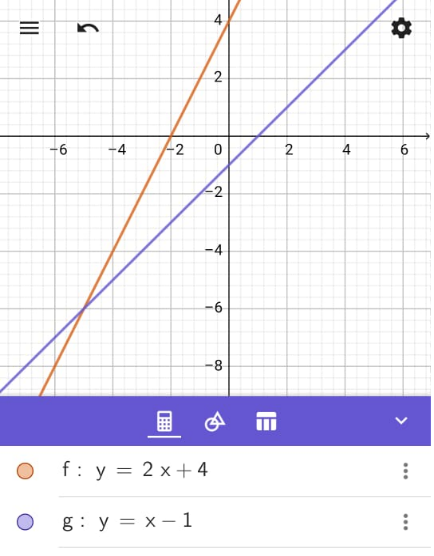
\includegraphics[width=150bp]{inequacoes1}
\end{figure}


\begin{enumerate}
\item Quais são as raízes de $f$ e de $g$?
\item Descreva a variação do \textit{sinal} dessas duas funções. 
\end{enumerate}

Toque em 
\includegraphics[height=.75cm]{inequacoes32} e em seguida em 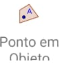
\includegraphics[height=.75cm]{inequacoes33}. Toque no eixo $x$, assim, você criou um ponto $(A)$ que se movimenta livremente sobre o eixo $x$.

Digite no campo entrada $(x(A),f(x(A)))$ e $(x(A),g(x(A)))$. O GeoGebra nomeará, automaticamente, esses pontos como $B$ e $C$.

\begin{figure}[H]
\centering

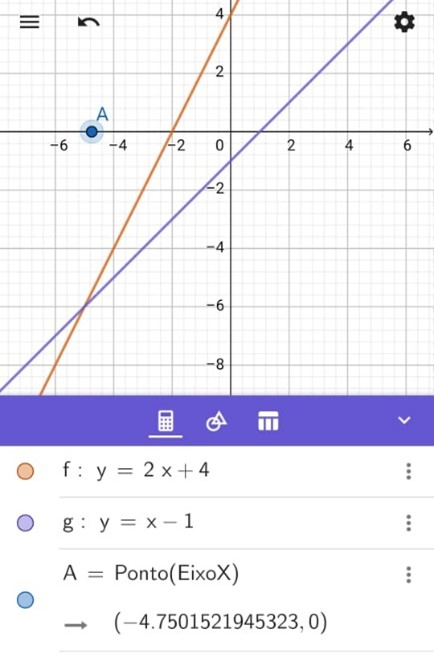
\includegraphics[width=150bp]{inequacoes2}
\end{figure}

Toque novamente em 
\includegraphics[height=.75cm]{inequacoes32} e, em seguida, em 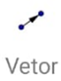
\includegraphics[height=.75cm]{inequacoes34}. Toque sequencialmente em $A$ e $B$ e, em seguida, em $A$ e $C$, criando os segmentos orientados $\overrightarrow{AB}$ e $\overrightarrow{AC}$. 

\begin{figure}[H]
\centering

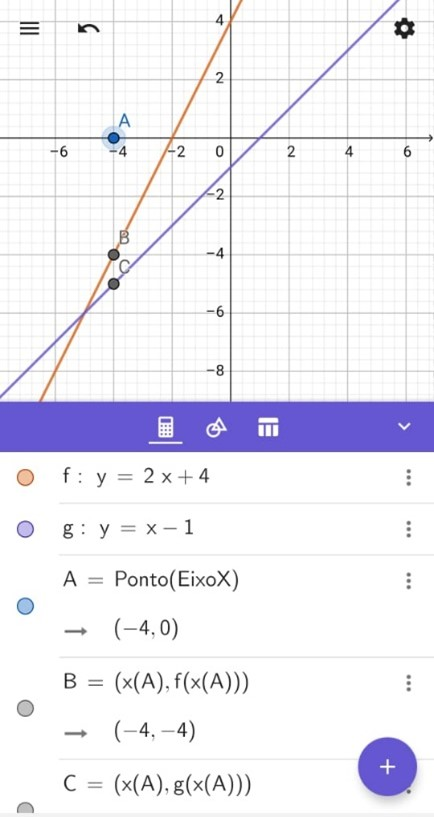
\includegraphics[width=150bp]{inequacoes3}
\end{figure}

Em seguida, ainda no menu  
\includegraphics[height=.75cm]{inequacoes32}, toque em 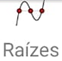
\includegraphics[height=.75cm]{inequacoes35} e, em seguida, em cada uma das duas retas que representam as funções $f$ e $g$, nessa ordem. Na tela você verá os pontos $E$ e $F$, raízes das funções $f$ e $g$, respectivamente.

\begin{figure}[H]
\centering

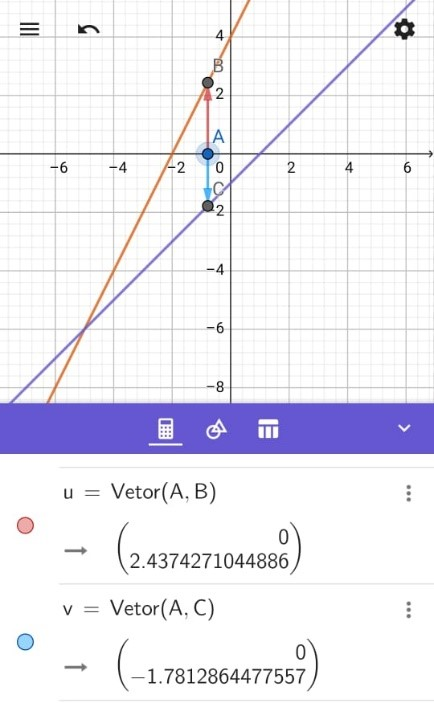
\includegraphics[width=150bp]{inequacoes4}
\end{figure}

\begin{enumerate}\setcounter{enumi}{2}
\item Movimente o ponto $A$ e descreva as possíveis posições relativas de $\overrightarrow{AB}$ e $\overrightarrow{AC}$
\item Em que intervalos $\overrightarrow{AB}$ e $\overrightarrow{AC}$ estão ambos abaixo do eixo $x$ (ou seja, para que valores de $x$ as funções $f$ e $g$ são negativas)?
\item Em que intervalos $\overrightarrow{AB}$ e $\overrightarrow{AC}$ estão ambos acima do eixo $x$ (ou seja, para que valores de $x$ as funções $f$ e $g$ são negativas)?
\item Em que intervalos $\overrightarrow{AB}$ e $\overrightarrow{AC}$ estão em sentidos opostos (ou seja, uma é positiva e outra é negativa)?
\item Vamos considerar agora a função $h(x) = f(x) \cdot g(x)$. Qual será o sinal de $h(x)$ quando $x < - 2$? E quando $x > 1$? E quando $-2 < x < 1$? E quando $x = -2$ ou $x = 1$? 
\item Faça o mesmo tipo de análise conduzida no item anterior para a função $q(x)=\dfrac{f(x)}{g(x)}$. 
\item A partir do que você percebeu acima (e sem desenvolver o produto), responda: qual a solução da inequação $f(x)\cdot g(x)<0$?
\item E qual a solução da inequação $\dfrac{f(x)}{g(x)}\geq0$ ? Os valores $x=-2$ e $x=1$ estão no conjunto solução dessa inequação? Justifique sua resposta.
\end{enumerate}

\ifdefined\prof
\begin{solucao}

\begin{enumerate}
\item A raiz de $f$ é $-2$ e de $g$ é $1$.
\item O sinal da função $f$ é negativo para valores menores que  $x=-2$, positivo valores maiores que $x=-2$ e nulo em $x=-2$;  a função $g$ é negativa para valores de $x$ menores que $1$; positiva para valores de $x$ maiores que $1$ e nula em $x = 1$.
\item Podem ambos estar abaixo do eixo $x$, ambos acima do eixo $x$ ou um abaixo e outro acima do eixo $x$.
\item Estão ambos abaixo do eixo $x$ para valores de $x$ menores que $-2$, raiz de $f$.
\item Estão ambos acima do eixo $x$ para valores de $x$ maiores que $1$, raiz de $g$.
\item Estão em sentidos opostos quando $x$ está entre $-2$ e $1$; aqui, $AB$ está acima do eixo $x$ (positivo) e $AC$ está abaixo do eixo $x$ (negativo).
\item Nesse caso, temos que o sinal de $h$ será positivo para valores de $x$ menores que $-2$ e para valores de $x$ maiores que $1$, pois nesse caso, o sinal das duas funções é o mesmo. Já quando $x$ é um valor entre $-2$ e $1$, o sinal de $h$ será negativo, pois nesse caso temos $f$ negativa e $g$ positiva. Em $x = -2$ ou em $x = 1$, como um dos fatores seria nulo, então temos que $h$ é nula.
\item Nesse caso, a situação é análoga ao item anterior, exceto pelo caso em que temos $x=1$ pois, nessa situação, $g(x)=0$, o que inviabiliza o quociente. Portanto, temos que $q$ é negativa quando $x$ está entre $-2$ e $1$ e positiva para valores de $x$ menores que $-2$ ou maiores que $1$. Em $x=-2, q$ será nula, pois teremos o quociente entre zero e um número negativo, o que resulta em zero.
\item Conforme vimos no item $(g)$, a função $h$ é negativa, estritamente, quando $x$ está entre $-2$ e $1$; logo, o conjunto solução dessa inequação é $]-2,1[$.
\item  Conforme vimos no item $(h)$ a função $q$ é positiva quando $x$ é menor que $-2$ ou quando $x$ é maior que $1$. No entanto, note que aqui a desigualdade está incluindo o zero; mas como precisaremos excluir o valor $1$ do domínio de $q$, então a solução será $]-\infty, -2]\cup ]1,+\infty[$
\end{enumerate}

\end{solucao}
\fi

\end{document}